\documentclass[aspectratio=169,12pt,t]{beamer}
\usetheme{default}
\usecolortheme{seahorse}
\usepackage[UTF8]{ctex}
\usepackage[version=4]{mhchem} %化学公式宏包
\usepackage{siunitx} %数字,单位宏包

%\setbeamertemplate{background}{\includegraphics[height=\paperheight]{bg.pdf}}
\setbeamertemplate{navigation symbols}{}   %取消导航条
\setbeamertemplate{footline}[frame number]    %页码
\setbeamerfont{frametitle}{size=\fontsize{16}{20}}  %标题
\setbeamerfont{framesubtitle}{size=\fontsize{10}{12}}  %副标题
\setlength{\parindent}{2em}      %段落缩进2字符
\linespread{1.2}

%---------------------突出本章标题--------------------------------------------
\AtBeginSection[]
{
	\begin{frame}{目录}
		\transfade%淡入淡出效果
		\tableofcontents[sectionstyle=show/shaded] %这几个参数我也不知道该如何准确地解释,反正它们最终的效果是突出显示当前章节,而其它章节都进行了淡化处理
		\addtocounter{framenumber}{-1}  %目录页不计算页码
	\end{frame}
}
%-------------------字体----------------------------------------------

\usefonttheme{serif}
\setmainfont{Times New Roman}
\usepackage{amsmath}
\usepackage{unicode-math}
\setmathfont{XITS Math}

%------------------封面-----------------------------------------------
\title{化学反应工程}
\subtitle{Chemical Reaction Engineering}
\author{张斌}
\institute[河北农业大学 理工系]{河北农业大学 理工系}
\date{\today}
%-----------------------------------------------------------------
\begin{document}

	%----------------------封面----------------------------------------
	\begin{frame}
		\titlepage
	\end{frame}
	%----------------------目录-------------------------------------------
	\begin{frame}
		\frametitle{目录}
		\tableofcontents
	\end{frame}




%------------------2.3 温度对反应速率的影响-----------------------
\section{2.3 温度对反应速率的影响}
\begin{frame}
	\frametitle{1 阿伦尼乌斯方程}
        在幂函数型速率方程中,以温度函数$f_1(T)$来体现温度对反应速率的影响。对于一定的温度,$f_1(T)$为定值,以反应速率常数$k$来表示。通常用阿伦尼乌斯方程来表示反应速率常数与温度的关系。
    $$k = A\exp(-E/RT) $$\\
    式中,$A$为指前因子;$E$为活化能;$R$为气体常数。
    \\k的物理意义:所有反应组分的浓度均为1时的反应速率。
    \\k的单位:与反应速率的表示方式、速率方程的形式、以及反应物系组成的表示方式有关。
        \\化学反应速率总是随着温度的升高而增加(极少数者例外)。
\end{frame}


\begin{frame}
	\frametitle{2 阿伦尼乌斯方程的其他形式}
	积分式
	$$\ln{k}=\ln{A}-E/RT$$\\
	以$\ln{k}$对$1/T$作图可得一直线,由直线的斜率可决定反应的活化能。
	\\~
	\\微分式
	$$\frac{\mathrm{d}\ln{k}}{\mathrm{d}T} =\frac{E}{RT^2}$$
	\\~
	\\定积分式
	$$\ln\frac{k_2}{k_1}=\frac{-E_a}{R}(\frac{1}{T_2}-\frac{1}{T_1})$$	
\end{frame}


\begin{frame}
	\frametitle{3 正逆反应活化能的关系}
	如果可逆反应的正逆反应速率常数均符合阿伦尼乌斯方程,则有
	$$\frac{\mathrm{d}\ln\overrightarrow{k}}{\mathrm{d}T} =\frac{\overrightarrow{E}}{RT^2}~~~~~~~~
	\frac{\mathrm{d}\ln\overleftarrow{k}}{\mathrm{d}T} =\frac{\overleftarrow{E}}{RT^2}~~~~\Rightarrow ~~~~\frac{\mathrm{d}\ln\overrightarrow{k}}{\mathrm{d}T}-\frac{\mathrm{d}\ln\overleftarrow{k}}{\mathrm{d}T}=\frac{\overrightarrow{E}-\overleftarrow{E}}{RT^2}$$
	\\由正逆反应速率常数关系式$\overrightarrow{k}/\overleftarrow{k}=K_c^{1/\nu}$两边取对数,得
	$$\frac{\mathrm{d}\ln\overrightarrow{k}}{\mathrm{d}T}-\frac{\mathrm{d}\ln\overleftarrow{k}}{\mathrm{d}T}=\frac{1}{\nu}\frac{\mathrm{d}\ln{K_p}}{\mathrm{d}T}$$
	\\又有范特霍夫方程$\frac{\mathrm{d}\ln{K_p}}{\mathrm{d}T}=\frac{\Delta{H_r}}{RT^2}$,则
	$$\overrightarrow{E}-\overleftarrow{E}=\frac{1}{\nu}\Delta{H_r}$$
	\\对于吸热反应,$\Delta{H_r}>0$,所以$\overrightarrow{E}>\overleftarrow{E}$;放热反应,$\Delta{H_r}<0$,$\overrightarrow{E}<\overleftarrow{E}$;
\end{frame}


\begin{frame}
	\frametitle{4 温度对可逆反应速率的影响}
	可逆反应的反应速率等于正逆反应速率之差,用组分A的转化率$X_A$来表示可写成:
	$$r=\overrightarrow{k}f(X_A)-\overleftarrow{k}g(X_A)$$
	\\对$T$求导,得
	$$(\frac{\partial r}{\partial T} )_{X_A}=f({X_A})\frac{\mathrm{d}\overrightarrow{k}}{\mathrm{d}T}-g({X_A})\frac{\mathrm{d}\overleftarrow{k}}{\mathrm{d}T}$$
	\\根据阿伦尼乌斯方程
	$$\frac{\mathrm{d}\ln\overrightarrow{k}}{\mathrm{d}T} =\frac{\overrightarrow{E}}{RT^2}~~~~\Rightarrow~~~~\frac{\mathrm{d}\overrightarrow{k}}{\mathrm{d}T}=\frac{\overrightarrow{k}\overrightarrow{E}}{RT^2}~~~~~~~~\frac{\mathrm{d}\overleftarrow{k}}{\mathrm{d}T}=\frac{\overleftarrow{k}\overleftarrow{E}}{RT^2}$$
	$$(\frac{\partial r}{\partial T} )_{X_A}=\frac{\overrightarrow{E}}{RT^2}\overrightarrow{k}f({X_A})-\frac{\overleftarrow{E}}{RT^2}\overleftarrow{k}g({X_A})$$
\end{frame}


\begin{frame}
	\frametitle{4.1 温度对可逆吸热反应速率的影响}
			$(\frac{\partial r}{\partial T} )_{X_A}=\frac{\overrightarrow{E}}{RT^2}\overrightarrow{k}f({X_A})-\frac{\overleftarrow{E}}{RT^2}\overleftarrow{k}g({X_A})$
	\\因为$r\ge 0$,所以$\overrightarrow{k}f({X_A})\ge \overleftarrow{k}g({X_A})$。
	\\对于可逆吸热反应,$\overrightarrow{E}> \overleftarrow{E}$,$(\frac{\partial r}{\partial T} )_{X_A}> 0$
	\\可逆吸热反应的速率总是随着温度的升高而增加。
	\centerline{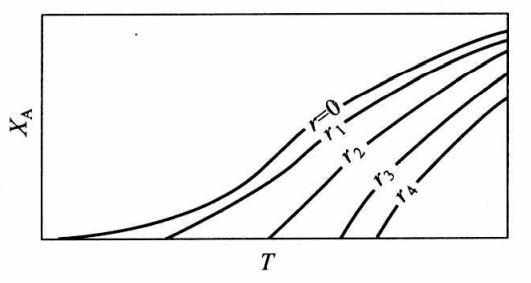
\includegraphics[height=3.8cm]{figs/fig2.2}}
	\centerline{\scriptsize{可逆吸热反应的反应速率与温度及转化率的关系($r_4>r_3>r_2>r_1$)}}
\end{frame}


\begin{frame}
	\frametitle{4.2 温度对可逆放热反应速率的影响}
	\begin{columns}[c]
	\column{7cm}
		$$(\frac{\partial r}{\partial T} )_{X_A}=\frac{\overrightarrow{E}}{RT^2}\overrightarrow{k}f({X_A})-\frac{\overleftarrow{E}}{RT^2}\overleftarrow{k}g({X_A})$$
		\\~~~~~~~~对于可逆放热反应,$\overrightarrow{E}< \overleftarrow{E}$,但$\overrightarrow{k}f({X_A})> \overleftarrow{k}g({X_A})$,所以
		\\$(\frac{\partial r}{\partial T} )_{X_A}> 0$;$(\frac{\partial r}{\partial T} )_{X_A}= 0$;$(\frac{\partial r}{\partial T} )_{X_A}< 0$
		\\~~~~~~~~可逆放热反应的速率随着温度的升高既可能增加,又可能降低,如图所示。
		\\~~~~~~~~图中曲线是在一定转化率下作出的,也叫等转化率线。
			\column{7cm}
		\centerline{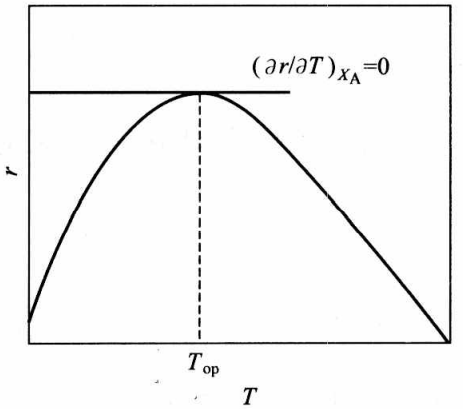
\includegraphics[height=4.5cm]{figs/fig2.3}}
		\centerline{\scriptsize{可逆放热反应的反应速率与温度的关系}}
		\\~~~~~~~~曲线的最高点$(\partial r/\partial T =0) $的温度叫做最佳温度$T_{\mathrm{op}}$。
	\end{columns}
\end{frame}


\begin{frame}
	\frametitle{4.3 可逆放热反应最佳温度曲线}
	\begin{columns}
		\column{7cm}
		反应速率极大点斜率为零,$(\frac{\partial r}{\partial T} )_{X_A}= 0$
		$$\overrightarrow{E}\overrightarrow{k}f({X_A})-\overleftarrow{E}\overleftarrow{k}g({X_A})=0$$
		$$\frac{\overrightarrow{E}\overrightarrow{A}\exp(-\overrightarrow{E}/RT_{\mathrm{op}})}{\overleftarrow{E}\overleftarrow{A}\exp(-\overleftarrow{E}/RT_{\mathrm{op}})}=\frac{g({X_A})}{f({X_A})}$$
		\\当反应达到平衡时,$$r=\overrightarrow{k}f(X_A)-\overleftarrow{k}g(X_A)=0$$
		$$\frac{g({X_A})}{f({X_A})}=\frac{\overrightarrow{k}}{\overleftarrow{k}}=\frac{\overrightarrow{A}\exp(-\overrightarrow{E}/RT_{\mathrm{e}})}{\overleftarrow{A}\exp(-\overleftarrow{E}/RT_{\mathrm{e}})}$$
				\column{7cm}
				将上式化简后两边取对数,整理后得				
		$$T_{\mathrm{op}}=\frac{T_{\mathrm{e}}}{1+\frac{RT_{\mathrm{e}}}{\overleftarrow{E}-\overrightarrow{E}}\ln\frac{\overleftarrow{E}}{\overrightarrow{E}}}$$
		\\平衡温度$T_{\mathrm{e}}$是转化率的函数,故最佳温度$T_{\mathrm{op}}$是转化率的隐函数。
		\\对应于任一转化率$X_A$,则必然有与其对应的平衡温度$T_{\mathrm{e}}$和最佳温度$T_{\mathrm{op}}$。
	\end{columns}
\end{frame}


\begin{frame}
	\frametitle{4.3 可逆放热反应最佳温度曲线}
	\begin{columns}[c]
		\column{7cm}
		\centerline{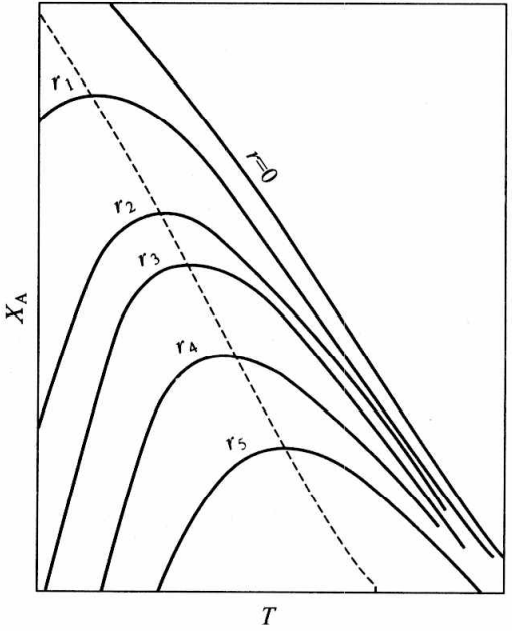
\includegraphics[width=5cm]{figs/fig2.4}}
		\centerline{\scriptsize{可逆放热反应的反应速率与温度及转化率的关系}}
		\column{7cm}
		曲线为等反应速率线,$r_5>r_4>r_3>r_2>r_1$
		\\$r=0$的曲线为平衡曲线,为反应进行的极限。
		\\连结所有等速率线上的极值点所构成的曲线(即图示虚线),叫做最佳温度曲线。
		\\对于可逆放热反应,如果从始至终按最佳温度曲线操作,那么整个过程将以最高的反应速率进行。
	\end{columns}
\end{frame}


\begin{frame}
	\frametitle{例}
	在实际生产中合成氨反应
	$$\mathrm{N_2}+1.5\mathrm{H_2}\rightleftharpoons \mathrm{NH_3}$$
	\\是在高温高压下采用熔融铁催化剂进行的。合成氨反应为可逆放热反应,故过程应尽可能按最佳温度曲线进行。现拟计算下列条件下的最佳温度:(1)在25.33MPa下,以3:1的氢氮混合气进行反应,氨含量为17\%;(2)其他条件同1,但氨含量为12\%;(3)把压力改为32.42MPa,其他条件同1。
	\\已知该催化剂的正反应活化能为$58.618×10^3\mathrm{J/mol}$,逆反应活化能为$167.48×10^3\mathrm{J/mol}$。平衡常数$K_\mathrm{p}\mathrm{(MPa^{-1})}$与温度$T$(K)及总压$p$(MPa)的关系如下:
	$$\log{K_p}=(2172.26 + 19.6478p)/T – (4.2405 + 0.02149p)$$
	
\end{frame}



\section{2.4 复合反应}
\begin{frame}{1 复合反应}
	在同一个反应物系中同时进行若干个化学反应时,称为复合反应。
	\\由于存在多个化学反应,物系中任一反应组分既可能只参与其中一个反应,也可能同时参与其中若干个反应。
	\\某一反应既可能是某一反应的反应物,又可能是另一反应的反应产物。
	\\在这种情况下,反应进程中该组份的反应量是所参与的各个化学反应共同作用的结果。
	\\我们把单位时间内单位体积反应混合物中某一组份$i$的反应量叫做该组份的转化速率($i$为反应物)或生成速率($i$为反应产物),并以符号$R_i$表示。
\end{frame}

\begin{frame}{2 反应组份的转化速率和生成速率}
	$R_i$应等于按组份$i$计算的各个反应的反应速率的代数和。
	$$R_i=\sum_{j=1}^{M} \nu_{ij}\overline{r}_j$$
	\\$\overline{r}_j$为第$j$个反应式的反应速率,乘以组份$i$在第$j$个反应中的化学计量系数$\nu_{ij}$,则得按组份$i$计算的第$j$个反应的反应速率。
	\\$R_i$值可正可负,若为正,表示该组份在反应过程中是增加的,$R_i$代表生成速率;若为负则情况相反,$R_i$表示消耗速率,或转化速率。
	\\转化速率或生成速率$R_i$与反应速率$r_i$的区别在于前者是针对若干反应,而后者则是对一个反应而言。
	\\如果只进行一个反应,$r_i=|R_i|$
\end{frame}

\begin{frame}{3 如何由$R_i$求$\overline{r}_j$}
	复合反应动力学实验测量得到的是各个反应综合的结果,即反应组分的生成速率或消耗速率。动力学研究最关心的是各个反应的反应速率,因之就存在一个如何由$R_i$求$\overline{r}_j$的问题。
	\begin{itemize}
		\item[\bullet ] 明确系统中有哪些反应,并分清主次。
		\item[\bullet ] 忽略次要反应,只考虑起主要作用的反应。
		\item[\bullet ] 设所要考虑的反应数目为M,通过实验测定不少于M个组分的生成速率或消耗速率。
		\item[\bullet ] 得到M个线性代数方程,解之得各个反应的反应速率$\overline{r}_j$。
	\end{itemize}
	~~~~~~~~应注意,这M个反应必须是独立反应。所谓独立反应是指这些反应中任何一个反应都不可能由其余反应进行线性组合而得到。
\end{frame}


\begin{frame}{4 独立反应数的确定}
	以甲烷水蒸汽转化反应为例
	$$\mathrm{CH_4+H_2O\rightleftharpoons CO+3H_2}$$
	$$\mathrm{CH_4+2H_2O\rightleftharpoons CO_2+4H_2}$$
	$$\mathrm{CO+H_2O\rightleftharpoons CO_2+H_2}$$
	\\其中只有两个是独立反应,因为其中总有一个反应可由其余两个线性组合得到,例如$(2)-(1)=(3),(1)+(3)=(2)$。
\end{frame}


\begin{frame}{4.1 通过化学计量系数矩阵得到独立反应数}
	对于化学计量系数矩阵A,其元素由全部5个反应组分在对应的3个化学反应式中的化学计量系数构成。
	$$\mathrm{CH_4~H_2~H_2O~CO~CO_2}$$
	$$\mathrm{A} = \begin{pmatrix}
	-1&  3&  -1&  -1& 0\\
	-1&  4&  -2&  0& 1\\
	0&  1&  -1&  -1& 1
\end{pmatrix}~~~~
\begin{matrix}
	(1)\\
	(2)\\
	(3)
\end{matrix}$$
	\\经初等变换后,求得矩阵A的秩$R(\mathrm{A})=2$,此时独立反应数等于矩阵的秩。
\end{frame}


\begin{frame}{4.2 通过原子系数矩阵得到独立反应数}
	在未知化学反应式的情况下,还可根据反应组分确定独立反应数。将反应式中所包含的全部元素种类,按分别出现在5个反应组分中的原子个数,写成原子系数矩阵B。
	$$\mathrm{CH_4~H_2~H_2O~CO~CO_2}$$
	$$\mathrm{A} = \begin{pmatrix}
		-1&  3&  -1&  -1& 0\\
		-1&  4&  -2&  0& 1\\
		0&  1&  -1&  -1& 1
	\end{pmatrix}~~~~~~ 
	\begin{matrix}
		\mathrm{C}\\
		\mathrm{H}\\
		\mathrm{O}
	\end{matrix}$$
	\\求得矩B的秩$R(\mathrm{B})=3$,此时的独立反应数等于反应组分数$-R(\mathrm{B})$
	$$5-3=2$$
	\end{frame}


\begin{frame}{5 复合反应的基本类型}
	复合反应包括三个基本类型:
	\begin{itemize}
		\item[\bullet ] 并列反应\par 反应系统中各个反应的反应组分各不相同
		\item[\bullet ] 平行反应\par 反应物完全相同而反应产物不相同或不全相同
		\item[\bullet ] 连串反应\par 一个反应的反应产物同时又是另一个反应的反应物
	\end{itemize}
	~~~~~~~~可逆反应亦属复合反应之列,但它可按单一反应的办法来处理,所以不将它包括在内。
\end{frame}


\begin{frame}{5.1 并列反应}
	$$\ce{A ->P}$$
	$$\ce{B ->Q}$$
	\\各个反应都可按单一反应来处理而得到相应的速率方程。
	\\任一个反应的反应速率不受其他反应的反应组分浓度的影响,但有些催化反应除外。
	\\因此,各个反应独立进行是并列反应的动力学特点。
	\\如果是变容过程,一个反应进行的速率会受到另一个反应速率的影响,如气相反应\ce{A ->P},\ce{2B ->Q},第二个反应会改变反应物系的体积,从而改变A和P的浓度,因之影响第一个反应的速率。
\end{frame}


\begin{frame}{5.2 平行反应}
	$$~~~\ce{A ->P}\qquad r_\mathrm{P}=k_1c_\mathrm{A}^\alpha$$
	$$\ce{\nu_{A}A ->Q}\qquad r_\mathrm{Q}=k_2c_\mathrm{A}^\beta$$
	\\如果我们的目的是生产P,则P称为{\color{red}目的产物(或主产物)},其它产物均称{\color{red}副产物}。生成主产物的反应称{\color{red}主反应},其它的均称为{\color{red}副反应}。
	\\研究复合反应的目标之一是加快主反应的速率,降低副反应的速率,以获得尽可能多的目的产物。通常用{\color{red}瞬时选择性}来评价主副反应速率相对大小。
	$$S=\mu_\mathrm{PA}\frac{\mathscr{R}_\mathrm{P}}{|\mathscr{R}_\mathrm{A}|}$$
	\\式中,$\mu_\mathrm{PA}$为生成1molP所消耗的A的mol数。用瞬时选择性这个词,是要表明其值随反应物系的组成及温度而变,它是一个瞬时值。
\end{frame}


\begin{frame}{5.2.1 浓度对平行反应瞬时选择性的影响}
	$$S=\frac{k_1c_\mathrm{A}^\alpha}{k_1c_\mathrm{A}^\alpha+|{\nu_\mathrm{A}}|k_2c_\mathrm{A}^\beta}=\frac{1}{1+\frac{k_2}{k_1}|{\nu_\mathrm{A}}|c_\mathrm{A}^{\beta -\alpha}}$$
	\\若温度一定,
\end{frame}
\section{2.5 反应速率方程的变换与积分}
\section{2.6 多相催化与吸附}
\section{2.7 多相催化反应动力学}
\section{2.8 动力学参数的确定}




\end{document}